\section{System Design}

In the previous chapter we focus on the system as a deployable \acrlong{mvp}. However, due to limitations of this project, we only implement a part of this \acrshort{mvp} to demonstrate the concept functionality -- we implement a prototype. The prototype demonstrates, how a FIDO key is used in the system to Authenticate a user and how this information is relayed to an external system to sign the user in. This chapter explains in more details selected prototype use cases and requirements. It then continues to describe the components of the prototype and high-level system flows.


% The main focus of this project and the very basis of the system is Authentication and Authorisation. One can argue that Access policy management is an integral part of the system, with which we agree, but for the purposes of the prototype this can be hardcoded and focus can be put upon implementation of Authentication and Authorisation components of the system which utilises \acrshort{fido}2 technology and \acrlong{oidc} +  OAuth standards. Therefore, the prototype will demonstrate employee's sign-in to external client system and opening of doors.

% In this section, the prototype to be implemented is described. Followed by the detail explanation of Use cases and Requirements associated with the prototype. This section further analyse the entities of the proposed system and their roles. Afterwards, we present high-level sequence diagrams of the system for the basic use cases. We explain what messages flow among the system components and how these represent the individual authentication and authorisation flows explained in the \href{sec:analysis}{Analysis section}. 

\subsection{Prototype Use Cases} \label{sec:design-prototype-usecases}
To demonstrate the functionality of the proposed \acrshort{acs} in practice, we select the most common uses of our system: signing in, passing a checkpoint and accessing a protected resource. These are represented by UC-1, UC-2, and UC-16 and are discussed further.

UC-1 and UC-2 include the authentication flow with FIDO, which is not used widely today in the combination of Online and \acrlong{pacs}, as discussed in Section~\ref{sec:analysis-authentication}. UC-16 (generalisation of UC-17 and UC-18) complements the sign-in process by providing information about the user and serving the protected resources to the client. These are essentially the use cases that an employee would encounter on a daily basis. The remaining use cases are more administrative and are not necessary to demonstrate the intended system functionality, therefore they are not discussed further.

On the following pages, detailed description of the use cases is provided for UC-1 (Table~\ref{tab:useCase_01}), UC-2 (Table~\ref{tab:useCase_02}), UC-17 (Table~\ref{tab:useCase_10}) and UC-18 (Table~\ref{tab:usecase-18-specs}).

\newgeometry{left=1.2cm,right=1.2cm,top=1cm,bottom=1cm,footskip=.4cm}
\begin{table}[htpb!]
    \footnotesize
    \onehalfspacing
    \centering
    \begin{tabular}{|c|p{15cm}|}
    \hline
    \cellcolor[HTML]{CBCEFB}\textbf{Name}&
    UC-1: Sign-in to a system
    \\
    \hline
    \cellcolor[HTML]{CBCEFB}\textbf{Description}&
    Employee signs-in to an internal or external client system with their enterprise digital identity using single-factor \acrshort{fido} physical key via \acrshort{usb} or \acrshort{nfc}; or \acrshort{fido} on a smartphone.
    \\
    \hline
    \cellcolor[HTML]{CBCEFB}\textbf{Primary actors}& 
    \textbullet~Employee
    \\
    \hline
    \cellcolor[HTML]{CBCEFB}\textbf{Secondary actors}& 
    \textbullet~Internal system, or \newline
    \textbullet~External system
    \\
    \hline
    \cellcolor[HTML]{CBCEFB}\textbf{Pre-conditions}&
    \vspace{-\topsep}
    \begin{itemize}[nolistsep, noitemsep, leftmargin=*]
        \item Employee has an enterprise digital identity assigned.
        \item Employee has previously registered at least one of the following authenticators:
        \begin{enumerate*}[label=(\roman*)]
            \item single-factor \acrshort{fido} physical key with \acrshort{usb} or \acrshort{nfc},
            \item \acrshort{fido} enabled smartphone.
        \end{enumerate*}
        \item Employee is in control of the previously registered authenticator.
        \item Employee does not have an active session with the given client on the given device.
        \item Policies have been set up that authorise the employee to access the client.\vspace*{-\baselineskip}
    \end{itemize}
    \\
    \hline
    \cellcolor[HTML]{CBCEFB}\textbf{Processing}& 
    \vspace{-\topsep}
    \begin{enumerate}[nolistsep, noitemsep, leftmargin=*]
        \item Employee launches the client application (either natively on the platform or in a web-browser). The client can be either internal system or external system. The sign-in process of the employee is the same in both cases. 
        \item Employee clicks on \textit{Sign-in}, \textit{Log-in} or similar button, or is redirected to sign-in automatically. A sign-in form appears.
        \item Employee enters their \acrlong{uid}.
        \item Employee is prompted to select their preferred authentication method: a physical key or a smartphone. If a physical key is selected, the employee is prompted to use their key with their device (depending on the make of the key and the device). If a smartphone is selected, the employee is prompted to navigate to a predefined website (enterprise-supplied authentication front end) on their smartphone, where they are prompted to authenticate with FIDO.
        \item Once the employee has been successfully authenticated, their attributes are checked against the existing policies for the system and the authorisation to access the system is verified.\vspace*{-\baselineskip}
    \end{enumerate}
    \\
    \hline
    \cellcolor[HTML]{CBCEFB}\textbf{Outcome}& 
    \vspace{-\topsep}
    \begin{itemize}[nolistsep, noitemsep, leftmargin=*]
    \item Employee signed-in and may begin to use the system, or
    \item Employee is denied to access the system because they could not be authenticated or are not authorised to access the given system.\vspace*{-\baselineskip}
    \end{itemize}
    \\
    \hline
    \cellcolor[HTML]{CBCEFB}\textbf{Post-conditions}&
    \textbullet~A session is created between employee's device and the system. Depending on the security settings, the employee might not need to sign in the next time when they use the system.
    \\
    \hline
    \end{tabular}
    \caption{Detailed specification of UC-1}
    \label{tab:useCase_01}
\end{table}
% 
% 
% 
% 
% 
\begin{table}[htpb!]
    \footnotesize
    \onehalfspacing
    \centering
    \begin{tabular}{|c|p{15cm}|}
    \hline
    \cellcolor[HTML]{CBCEFB}\textbf{Name}& 
    UC-2: Pass through a physical checkpoint
    \\
    \hline
    \cellcolor[HTML]{CBCEFB}\textbf{Description}& 
    Employee authenticate themselves to \acrlong{pacs} with their enterprise digital identity, using a \acrshort{fido} physical key via \acrshort{nfc} or with \acrshort{fido} on their smartphone.
    \\
    \hline
    \cellcolor[HTML]{CBCEFB}\textbf{Primary actors}&
    \textbullet~Employee
    \\
    \hline
    \cellcolor[HTML]{CBCEFB}\textbf{Secondary actors}&
    \textbullet~\acrlong{pacs}
    \\
    \hline
    \cellcolor[HTML]{CBCEFB}\textbf{Pre-conditions}&
    \vspace{-\topsep}
    \begin{itemize}[nolistsep, noitemsep, leftmargin=*]
        \item Employee has an enterprise digital identity assigned.
        \item Employee has previously registered at least one of the following authenticators:
         \begin{enumerate*}[label=(\roman*)]
            \item single-factor \acrshort{fido} physical key with \acrshort{usb} or \acrshort{nfc},
            \item \acrshort{fido} enabled smartphone.
         \end{enumerate*}
         \item Policies have been set up that authorise the employee to pass the given checkpoint.\vspace*{-\baselineskip}
     \end{itemize}
    \\
    \hline
    \cellcolor[HTML]{CBCEFB}\textbf{Processing}&
    \vspace{-\topsep}
    \begin{enumerate}[nolistsep, noitemsep, leftmargin=*]
        \item Employee approaches the checkpoint and the \acrshort{pacs} reader device mounted in vicinity.
        \item Employee swipes their physical FIDO key at the reader device to identify and authenticate themselves; or
        \item Employee indicates at the reader device that they wish to use smartphone to identify and authenticate themselves. They visit a special website (enterprise-supplied authentication front end), where they input the checkpoint ID and then authenticate using FIDO on the smartphone. 
        \item Once the system has authenticated the employee, it checks whether the policy permits the employee to pass the given checkpoint.\vspace*{-\baselineskip}
    \end{enumerate}
    \\
    \hline
    \cellcolor[HTML]{CBCEFB}\textbf{Outcome}&
    \vspace{-\topsep}
    \begin{itemize}[nolistsep, noitemsep, leftmargin=*]
    \item The checkpoint allows the employee to pass through, if the authentication was successful and policy permits access; or
    \item The access is denied and the employee is informed about the denial.\vspace*{-\baselineskip}
    \end{itemize}
    \\
    \hline
     \cellcolor[HTML]{CBCEFB}\textbf{Post-conditions}&\textbullet~Access attempt is logged in the system logs.\\
     \hline
    \end{tabular}
    \caption{Detailed specification of UC-2}
    \label{tab:useCase_02}
\end{table}
% 
% 
% 
% 
% 
\begin{table}[htpb!]
    \footnotesize
    \onehalfspacing
    \centering
    \begin{tabular}{|c|p{15cm}|}
    \hline
    \cellcolor[HTML]{CBCEFB}\textbf{Name}&
    UC-17: Access user's protected resources 
    \\
    \hline
    \cellcolor[HTML]{CBCEFB}\textbf{Description}&
    External systems might need to read or modify user's protected resources, such as files, emails, calendar entries, or others, to fulfil their function.
    \\
    \hline
    \cellcolor[HTML]{CBCEFB}\textbf{Primary actors}&
    \textbullet~External client
    \\
    \hline
    \cellcolor[HTML]{CBCEFB}\textbf{Secondary actors}&
    None
    \\
    \hline
    \cellcolor[HTML]{CBCEFB}\textbf{Pre-conditions}&
    \vspace{-\topsep}
    \begin{itemize}[nolistsep, noitemsep, leftmargin=*]
        \item A client connection between the external system and the \acrshort{acs} has been established.
        \item The policy permits the system to access user's protected resources.
        \item The user has previously signed in to the external system.\vspace*{-\baselineskip}
    \end{itemize}
    \\
    \hline
    \cellcolor[HTML]{CBCEFB}\textbf{Processing}&
    \vspace{-\topsep}
    \begin{enumerate}[nolistsep, noitemsep, leftmargin=*]
        \item The \acrshort{acs} verifies that the external system has been registered and has been assigned a client ID.
        \item The \acrshort{acs} verifies that the user is signed in or has previously singed in to the external system. This can be demonstrated with a refresh token.
        \item The \acrshort{acs} verifies that the policy permits the external system to access user's protected resources.
        \item If the previous conditions are met, the \acrshort{acs} issues an access token to the External client. The external client uses this token when querying the system for user's resources. The validity of the token is time bound and can be only used to request resources about the user it has been issued for.\vspace*{-\baselineskip}
    \end{enumerate}
    \\
    \hline
    \cellcolor[HTML]{CBCEFB}\textbf{Outcome}&
    \vspace{-\topsep}
    \begin{itemize}[nolistsep, noitemsep, leftmargin=*]
    \item The external system can read or modify user's resources, after it has successfully presented a valid access token; or
    \item Access was denied and the external system cannot manipulate user's protected resources.\vspace*{-\baselineskip}
    \end{itemize}
    \\
    \hline
     \cellcolor[HTML]{CBCEFB}\textbf{Post-conditions}&
     \textbullet~The access token cannot be used for other user's resources, or after it's validity has expired.
     \\
     \hline
    \end{tabular}
    \caption{Detailed specification of UC-17}
    \label{tab:useCase_10}
\end{table}
% 
% 
% 
% 
% 
\begin{table}[htpb]
    \footnotesize
    \onehalfspacing
    \centering
    \begin{tabular}{|c|p{15cm}|}
    \hline
    \cellcolor[HTML]{CBCEFB}\textbf{Name}&
    UC-18: Access enterprise protected resources
    \\
    \hline
    \cellcolor[HTML]{CBCEFB}\textbf{Description}&
    External systems might need to read or modify protected resources owned by the enterprise (and which are not owned by any single user) to fulfil their function.
    \\
    \hline
    \cellcolor[HTML]{CBCEFB}\textbf{Primary actors}&
    \textbullet~External system
    \\
    \hline
    \cellcolor[HTML]{CBCEFB}\textbf{Secondary actors}&
    None
    \\
    \hline
    \cellcolor[HTML]{CBCEFB}\textbf{Pre-conditions}&
    
    \vspace{-\topsep}
    \begin{itemize}[nolistsep, noitemsep, leftmargin=*]
        \item A client connection between the external system and the \acrshort{acs} has been established and a client secret has been issued to the external system.
        \item The client acting on behalf of the external system is web-server based.
        \item The policy permits the access to the protected resources.\vspace*{-\baselineskip}
    \end{itemize}
    \\
    \hline
    \cellcolor[HTML]{CBCEFB}\textbf{Processing}&
    \vspace{-\topsep}
     \begin{enumerate}[nolistsep, noitemsep, leftmargin=*]
        \item The \acrshort{acs} verifies the client's client ID and client secret.
        \item The \acrshort{acs} verifies that the policy permits the external system to access enterprise protected resources.
        \item If the conditions are met, the \acrshort{acs} issues an Access Token to the External system client. The client presents this access token, when it is manipulating the protected resources. The access token has a limited validity and cannot be used for any other than requested resources, or after it's validity period has elapsed.\vspace*{-\baselineskip}
     \end{enumerate}
    \\
    \hline
    \cellcolor[HTML]{CBCEFB}\textbf{Outcome}&
    \vspace{-\topsep}
    \begin{itemize}[nolistsep, noitemsep, leftmargin=*]
        \item The external client obtained an access token and presented it in the request to manipulate the protected resource; or
        \item The external client has been denied access to the protected resources.\vspace*{-\baselineskip}
     \end{itemize}
    \\
    \hline
     \cellcolor[HTML]{CBCEFB}\textbf{Post-conditions}&
     \textbf~The access token cannot be used, after it's validity has expired.
     \\
     \hline
    \end{tabular}
    \caption{Detailed specification of UC-18}
    \label{tab:usecase-18-specs}
\end{table}
\restoregeometry
\subsection{Prototype Requirements}\label{sec:design-prototype-requirements}

Based on the use cases highlighted in the previous section, we describe the requirements necessary to implement these use cases. Naturally, all requirements linked with given use cases should be implemented. The following requirements are linked to the selected use cases: RQ-1, RQ-2, RQ3, RQ-4, RQ-5, RQ-18 and RQ-19. These requirements are selected to be implemented in the prototype and drive the design choices behind the system architecture. 

% TODO describe selected Requirements

% \begin{table}[H]
%     \footnotesize
%     \onehalfspacing
%     \centering
%     \begin{tabular}{|c|p{15cm}|}
%     \hline
%     \cellcolor[HTML]{CBCEFB}\textbf{ID}&\cellcolor[HTML]{CBCEFB}\textbf{Description}\\
%     \hline
%     RQ-1&User must be able to authenticate with single-factor cryptographic device based on FIDO2 to use their enterprise digital identity.\\
%     \hline
%     RQ-2&User must be able to authenticate with smartphone using FIDO2 flow to use their enterprise digital identity.\\
%     \hline
%     RQ-4&User must be able to sign-in to external client system with their enterprise digital identity.\\
%     \hline
%     RQ-5&User must be able to open a door with their enterprise digital identity.\\
%     \hline
    %     % RQ-19&\textbf{External client system must be able to access protected resources, when authorised to do so.}\\
%     RQ-18&External client system must be able to access protected resources if permission granted.\\
%     \hline
%     RQ-19&External client system must be able to obtain grant permission.\\
%     \hline
%     \hline
%     RQ-20&Authentication to PACS using enterprise digital identity must be comparably fast to traditional RFID access cards (order of milliseconds to seconds).\\
%     \hline
%     % RQ-21&\textbf{External system must be able to access protected resources.}\\
%     % \hline
%     RQ-21&The system must use OIDC + OAuth for Authentication and Authorisation.\\
%     \hline
%     RQ-22&The system must use XACML for Identity and Access management\\
%     \hline
%     \end{tabular}
%     \caption{List of functional requirements \#1, \#2, \#4, \#5, \#18, \#19 and non-functional requirements \#20, \#21, \#22 for the prototype.}
%     \label{tab:prototype-requirements}
% \end{table}
\subsection{Components}
To best design the architecture of our system, we must first understand the different actors and their roles. In the FIDO2, OAuth and \acrshort{oidc} specifications there is a degree of ambiguity -- problem being, that while each specification explains details in its own context, the link to other parts of an \acrshort{acs} are not obvious. In this section we identify components of our system and clear this ambiguity by drawing the borders of each specification within our system.

The external and internal systems are represented jointly as a \textit{Requester}. Requester is a system that is attempting to sign the user in, or access the protected resource. At the core of the proposed system is an \textit{\acrfull{aaserver}}, which carries out most of the authentication and authorisation tasks. The \acrshort{aaserver} consults with the User Directory and the  \acrfull{pdp}. To aid external systems retrieve information about users, the UserInfo endpoint translates the requests from the external systems to User Directory queries. Similarly, the Resource Endpoint provides access to the internal protected resources for the external systems. Both the UserInfo Endpoint and the Resource Endpoint are accessible from the public internet and lie on the boundary of the online security perimeter.

Figure~\ref{fig:data-flow-diagram} presents the high-level view of these components and their interactions. In the next sections we describe these components in more detail.

% TODO update figure
\begin{figure}[ht]
    \centering
    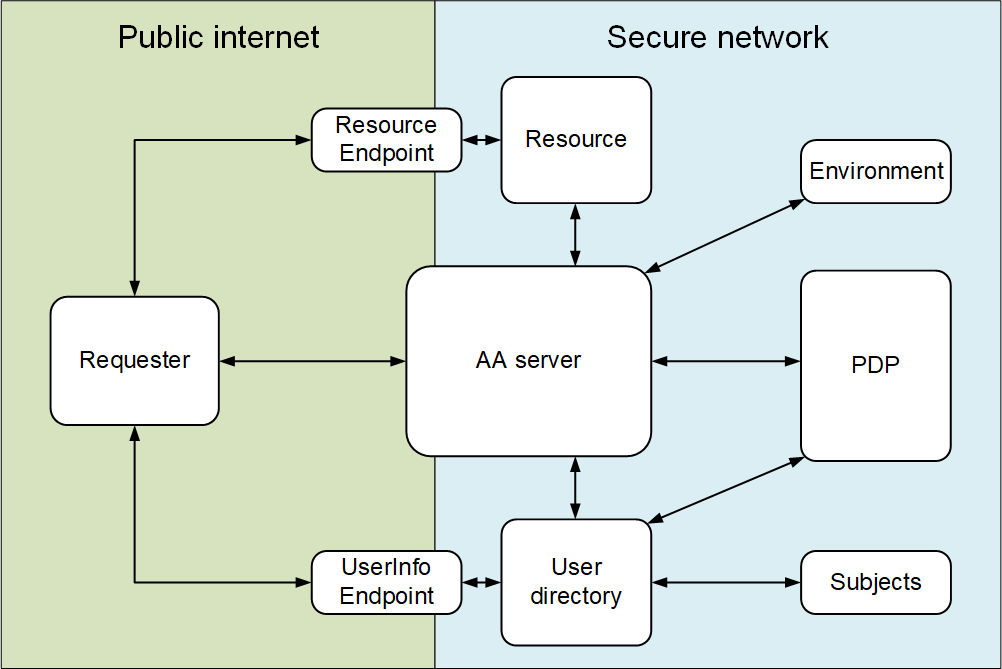
\includegraphics[width=.85\textwidth]{data-flow-diagram}
    \caption{High-level overview of system components and their interactions. The left side of the figure represents unsecured, public internet. The right side represents the security perimeter of the enterprise, which is not accessible from the public internet.}
    \label{fig:data-flow-diagram}
    % TODO check figure margins when outputed as PDF
\end{figure}

\subsubsection{Requester} 
Requester is the system or application that is requesting access to protected resources on behalf of the user. Typically, this would be an internal or external client application, or a \acrshort{pacs}.

Client application is the business application the user wishes to use. If this is an internal application, it sits within the security perimeter and has direct access to the protected resources. However, it still needs to authenticate the user and verify that the user is authorised to access these resources.

If the client application is is an external application, it also typically requires that the user is authenticated and is authorised to use this application. Furthermore, it may require access to user's own resources on their behalf (e.g. user's files) and access to enterprise-owned resources on it's own behalf (e.g. list of departments).
    
The client application can be either of the three client types that are recognised by the OAuth specification~\cite{Hardt2012TheFramework} -- web-based application (running on a web server), user-agent-based application (downloaded from the web server, but executed locally) or a native application. Examples of client application are Slack, Salesforce, ServiceNow or Zendesk.

The \acrshort{pacs} can also be a requester. Similarly as an internal application, it sits within the security perimeter. It needs to authenticate the users and evaluate whether the user is authorised to pass beyond a certain point in a facility.

\subsubsection{User agent}
User agent does not act on its own, but instead hosts web-based and user-agent-based applications. It interacts with the user during login and authentication by displaying login forms and communicating with the physical authenticator device via the CTAP2 protocol\footnotemark. It is typically a web browser. Principally, it could be both desktop- and mobile-based (currently only on the Android mobile platform). 
% 
\footnotetext{In the FIDO2 terminology, the user agent would be called the \textit{client} or \textit{client device}.}

Examples of user agents are Chrome, Mozilla, Microsoft Edge.

\subsubsection{Authentication and Authorisation Server} 
The \acrfull{aaserver} is the core of the proposed access control system. As the name suggests, it handles the authentication and authorisation of the users. It communicates with the User Agent, the Requester, the User Directory and the \acrshort{pdp}.
    
\paragraph{User access request}
The \acrshort{aaserver} authenticates the user during sign in, before they can use the client application, or during physical access control. This flow is activated by a \textit{User access request} from the Requester. If the Requester is a client application, the \acrshort{aaserver} supplies a login form. If the Requester is a \acrshort{pacs}, the login form is omitted to increase the speed of the process. The \acrshort{aaserver} then communicates with the Requester, the User Directory and, optionally with the Authentication front end until the user has been authenticated (this communication is described in detail in Section~\ref{sec:access-control-flows}).

After authentication, the \acrshort{aaserver} proceeds to verify that the user is authorised to access the requested resource. It supplies the necessary information to the \acrshort{pdp} and receives a response with the policy decision.

If the OAuth + \acrshort{oidc} flow is required and the \acrshort{pdp} issued an `Allow access' decision, the \acrshort{aaserver} continues the process with the requester until an access token and/or ID token are issued. If the \acrshort{pdp} issued a `Deny access' decision, the \acrshort{aaserver} informs the Requester that the access has been denied and does not issue the access token or ID token. 

If the OAuth and \acrshort{oidc} are not required (when the requester is an internal application or a \acrshort{pacs}), the \acrshort{aaserver} simply forwards the policy evaluation decision to the requester.

\paragraph{Client access request}
When a Requester requires access to protected resources on its own behalf, the user authentication flow is skipped. Instead, the Requester begins the process by sending a \textit{Client access request} to the \acrshort{aaserver}. The client then authenticates using its own set of credentials, using the client credential grant type, as defined by~\cite{Hardt2012TheFramework}. 

The \acrshort{aaserver} verifies the access policy for the Requester and if the Requester is authorised to access the protected resources, it issues an access token.

The client access request can only be sent by a web-based client (which runs on a server), since native and user-agent-based clients cannot guarantee the security of the client credentials.

\bigskip \noindent
Example of a similar system is Azure AD, discussed in Section~\ref{sec:online-access-control} or ForgeRock Identity Platform\footnotemark.
% 
\footnotetext{\url{https://www.forgerock.com/resources/view/63280622/product-brief/forgerock-identity-platform.pdf}, accessed 10 April 2019.}
    
\subsubsection{Authentication Front End}
The Authentication front end is used during user authentication, when the user selects to authenticate using FIDO2 on a smartphone. The Authentication Front End is a middle layer between the \acrshort{aaserver} and the smartphone OS, which handles the CTAP2 protocol, and moderates the communication between these two parties.

It receives Authentication Assertions (as defined by~\cite{Balfanz2019Web1}) from the \acrshort{aaserver} and presents these to the smartphone OS, which handles the signing process. Once signed, the Authentication Front End returns the assertions to the \acrshort{aaserver}.

The Authentication Front End could be a native application, running directly on the smartphone OS, but could also be a web page, if the browser is capable of relying the Authentication assertions to the OS\footnotemark. In our proposed system, this is a webpage, to offer more convenient access from a smartphone (without installation).
% 
\footnotetext{For example Chrome on Android supports the use of WebAuthn and CTAP2~\cite{ChromePlatformStatus2018SupportAPI}.}

\subsubsection{User Directory}
% TODO check consistent use accross report
The User Directory is a directory service that stores user attributes and can be accessed by the internal systems. In the proposed \acrshort{acs}, the User Directory is used to supply attributes about users for authentication and policy evaluation purposes. It also serves attributes to the UserInfo endpoint, when queried.

In addition to standard user attributes (such as name, email, office phone, job title etc.), the user directory stores details about user's authenticators -- the \texttt{credentialPublicKey}(as defined by~\cite{Balfanz2019Web1} -- authenticator's public key). This entry is created when the authenticator is first registered (UC-5) and is used to verify whether the credential challenge for a particular user was signed by an authenticator belonging to this user. Further authenticator details stored in the directory could be the signature counter or a user-defined authenticator name.

The User Directory interacts with the \acrshort{aaserver} when it supplies authenticator challenges and verifies authenticator challenge responses. It further interacts with the \acrshort{pdp} where it supplies user attributes, if these are required by the \acrshort{pdp} to evaluate the policy.

Examples of a user directory would be Active Directory\footnote{Active Directory by Microsoft is a subset of Azure AD described in Section~\ref{sec:online-access-control} on page~\pageref{sec:online-access-control}.} or the Apache Directory\footnotemark.
% 
\footnotetext{\url{https://web.archive.org/web/20190407171447/https://directory.apache.org/}, accessed 07 April 2019.}
    
\subsubsection{Policy Decision Point}
The \acrfull{pdp} determines whether a given user or Requester is authorised to access a protected resource. The \acrshort{pdp} stores the policies and when queried by the \acrshort{aaserver}, it evaluates the relevant policy and issues an evaluation decision.

It evaluates the policy based on user/Requester attributes, and optionally, additional context information. Some of these attributes are supplied by the \acrshort{aaserver} in the query. If these attributes are not sufficient to evaluate a policy, the \acrshort{pdp} can request additional information from the User Directory or the \acrshort{aaserver}.

As specified by RQ-22, \acrshort{xacml} is used to evaluate access policies. The \acrshort{pdp}, described by the \acrshort{xacml} specification~\cite{OASISStandard2013EXtensible3.0}, cannot operate on its own. Instead it communicates with other components to enforce the policy on the requester. The mapping of the proposed system components to the \acrshort{xacml} context is illustrated in Figure~\ref{fig:xacml-use}, Appendix~\ref{sec:xacml-use} on page~\pageref{fig:xacml-use}.

Example of a solution that implements \acrshort{pdp} functionality is \href{sec:online-access-control}{Azure AD} or WSO2 Identity Server\footnotemark.
% 
\footnotetext{\url{https://web.archive.org/web/20190407180021/https://docs.wso2.com/display/IS570/WSO2+Identity+Server+Documentation}, accessed 07 April 2019.}
    
\subsubsection{Resource Endpoint}
The Resource Endpoint serves the external clients. This endpoint is the gateway for the external application to access the protected enterprise resources. These resources are divided into scopes and the client must present a valid access token for the scope it is attempting to access. The endpoint must verify the validity of the presented token, before it serves the resource. The scopes are defined as \acrshort{api}s, specifying the form of the request and response messages.
    
\subsubsection{UserInfo Endpoint}
The UserInfo endpoint is a component as defined in~\cite{Sakimura2014Final:1}. It serves claims about user attributes to the external clients. The client must present a valid access token to receive the attributes of the associated user. The UserInfo Endpoint serves as an access point for clients outside the security perimeter, but it does not store any user attributes itself. Instead, it queries the User Directory for any requested attributes every time such request is received.

\bigskip \noindent
Not all of the mentioned components are necessarily different physical entities, but we list them here separately as they perform a different function are logically independent. In the following section, we describe the interactions between these components.
\subsection{Access control flows}
% NAME? "System flow example(s)

The access control flow of the proposed system can be broken down into three stages:
\begin{enumerate*}[label=(\roman*)]
    \item \textit{Authentication},
    \item \textit{Access Policy Evaluation} and
    \item \textit{Accessing protected resource}.
\end{enumerate*}
These stages can be identified in every use case of the system, although the flow in each stage is adapted to the given use case.

\subsubsection{Authentication}
In this stage, the user identifies and authenticates themselves to the \acrshort{aaserver}. This is the first stage of the access control flow and is only preceded by the user clicking a login button or approaching a door. The authentication is done via the FIDO2 protocol, but the flows during this stage are different during online login and when opening a door.

\paragraph{Authenticating online} During online authentication the user uses a browser or a native client application to communicate with the \acrshort{aaserver}. When the user clicks a login button, the client application redirects them to the login page, supplied by the \acrshort{aaserver}. The user agent/native client application needs to send a `Access request' message to the server, which contains these parameters: the \texttt{client\_id}, the callback URL, the requested scopes (and if the client is a native application, also the \acrshort{pkce} code challenge). The \texttt{client\_id} is immediately verified by the \acrshort{aaserver}. All variables are temporarily saved for use later in the process. 

The \acrshort{aaserver} provides a login form back to the requesting party. User enters their \acrshort{uid} into this form and chooses the authenticator they wish to use (physical key or smartphone). The filled form is then send back to the \acrshort{aaserver}. The server requests a login challenge for this \acrshort{uid} from the User directory. The User directory looks up the \acrshort{uid} in the user database and generates an Authentication assertion\footnotemark to be signed by the user's authenticator.
% 
\footnotetext{As defined by the WebAuthn specification: \url{https://www.w3.org/TR/webauthn/\#dictdef-publickeycredentialrequestoptions}, accessed 08 April 2019}

If the user selected physical key as their authenticator, the Authentication assertion is then forwarded back to the user agent/native application that made the initial access request. If the user selected smartphone, the the Authentication assertion is forwarded to the Authentication front end. Once the signed assertion is received, the \acrshort{aaserver} forwards it to the User directory. User directory verifies that the signature was made by either of the public keys, associated with the \acrshort{uid}. The User directory then informs the \acrshort{aaserver} about the outcome of this verification. 

In the last step of the Authentication stage, the \acrshort{aaserver} issues a signed and encrypted \acrshort{jwt} to the user agent/Authentication front end. This \acrshort{jwt} can be sent in the initial Access request and the remaining steps of the authentication stage are then skipped. The purpose of this is to avoid repeated authentication prompts to the user in a short time span (a couple of hours). Once the user authenticates using an authenticator on certain user agent, we do not need to prompt authentication on the same user agent again, until the validity of the \acrshort{jwt} has expired.

If a \acrshort{aaserver} receives a valid \acrshort{jwt} in the Access request, it does not carry out further authentication steps and proceeds directly to the Access policy evaluation stage. If the received \acrshort{jwt} is expired or otherwise invalid, the regular process described above applies.

\subsubsection{Access Policy Evaluation}

*tune of pink panther*
TO DO, TODO, TODO, TODO, TODOOOO....